% Package
\documentclass[11pt]{article}

\usepackage{amsmath}
\usepackage{cite}
\usepackage{graphicx}

\title{ADP Aufgabe 1, Abgabe 1}
\author{Team 1\\Hugo Protsch, Justin Hoffmann}

% Document
\begin{document}

    \maketitle


    \section{Formales}\label{sec:Formales}

    %! suppress = MissingLabel

    \subsection{Aufgabenaufteilung}
    Die Entwürfe wurden zusammen entwickelt.
    %! suppress = MissingLabel

    \subsection{Quellenangaben}
    -- Nicht zutreffend --

    %! suppress = MissingLabel

    \subsection{Bearbeitungszeitraum}
    Für die Bearbeitung haben wir in etwa 6 bis 8 Stunden benötigt.
    %! suppress = MissingLabel

    \subsection{Aktueller Stand}
    Die Entwürfe sind fertig gestellt und müssen Implementiert werden.

    %! suppress = MissingLabel

    \subsection{Änderungen des Entwurfes}
    -- Nicht zutreffend --


    \section{Entwürfe}\label{sec:entwürfe}

    \subsection{InitBT}
    Liefert einen leeren Baum. Entwurf ist trivial.

    \subsection{IsEmptyBT}
    Prüft einen Baum auf Leerheit. Entwurf ist trivial.

    \subsection{IsBt}

    \begin{center}
        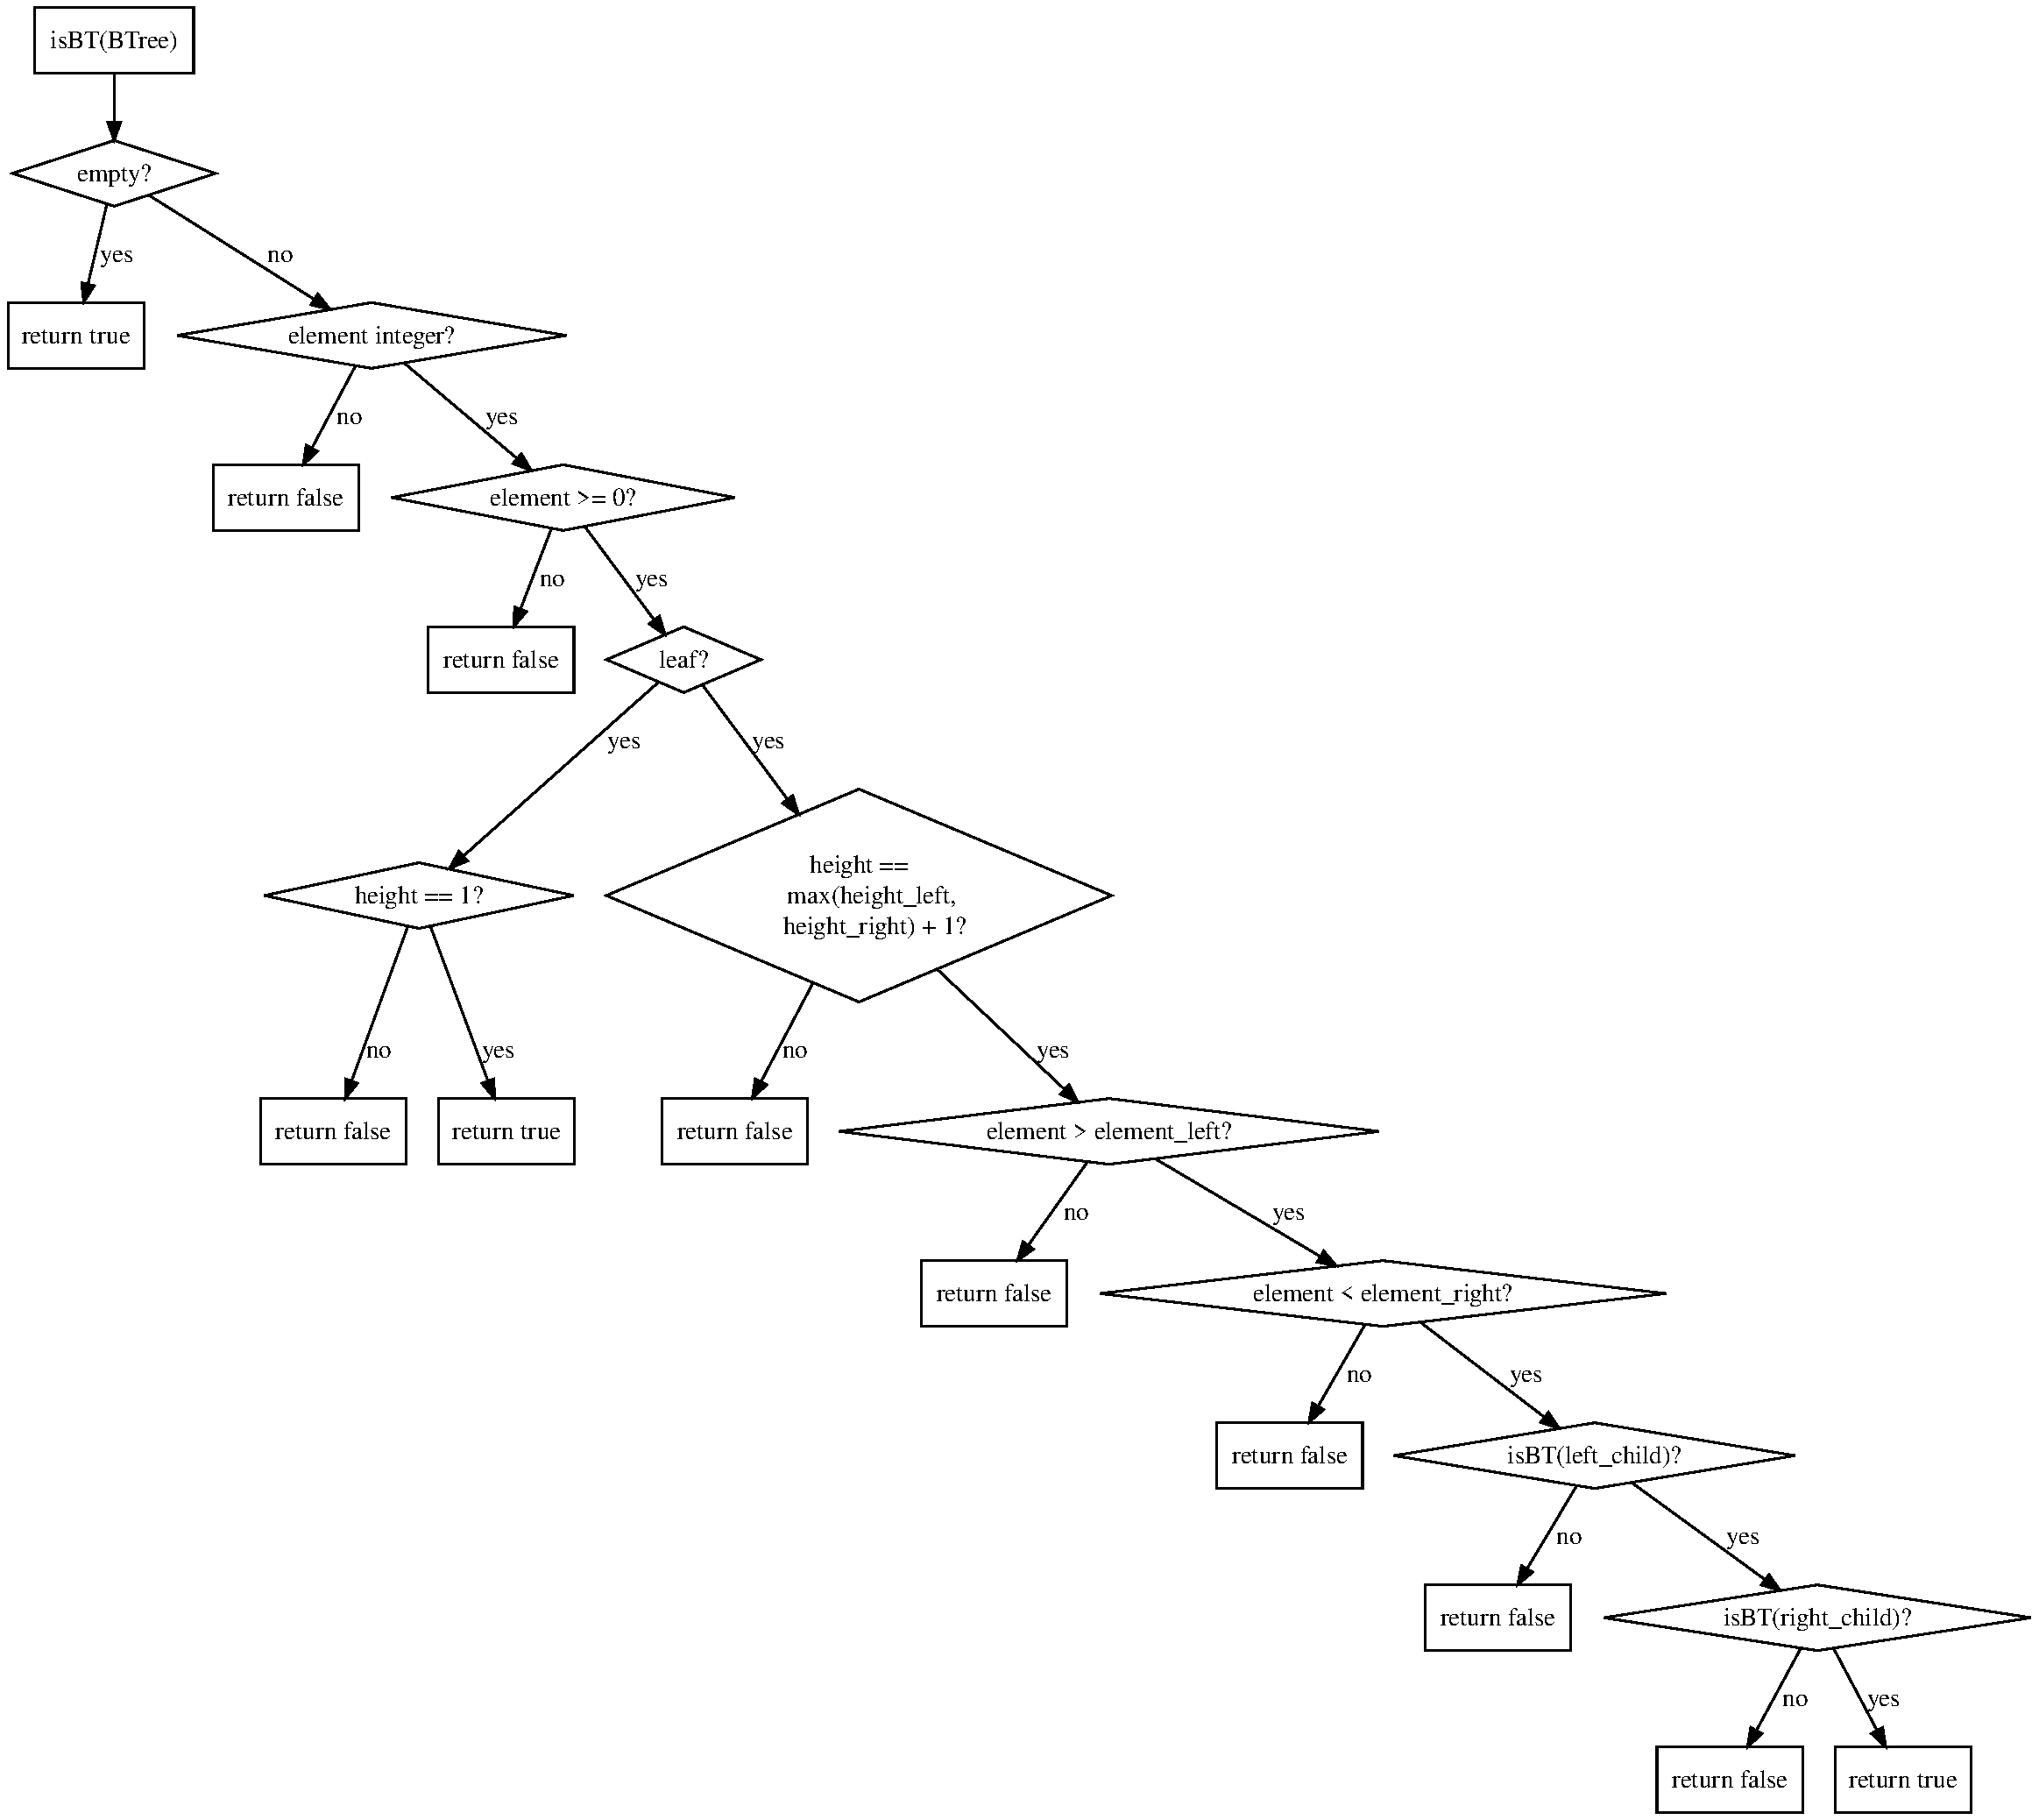
\includegraphics[width=1.2\columnwidth] {isBt}
    \end{center}

    Prüft die vorgegebenen Rahmenbedingungen eines übergebenen
    Baums. Hierbei werden alle Wahrheitswerte der verschiedenen
    Vorgaben von jedem Knote miteinander in einen logischen
    Zusammenhang gebracht.

    \subsection{EqualsBT}
    Prüft auf semantische Gleichheit zwischen zwei Bäumen.
    Entwurf ist ebenfalls trivial, da die inOrderBT-Funktion
    auf beide Bäume angewendet wird und die resultierenden Listen verglichen werden.

    \subsection{InsertBT}

    \begin{center}
        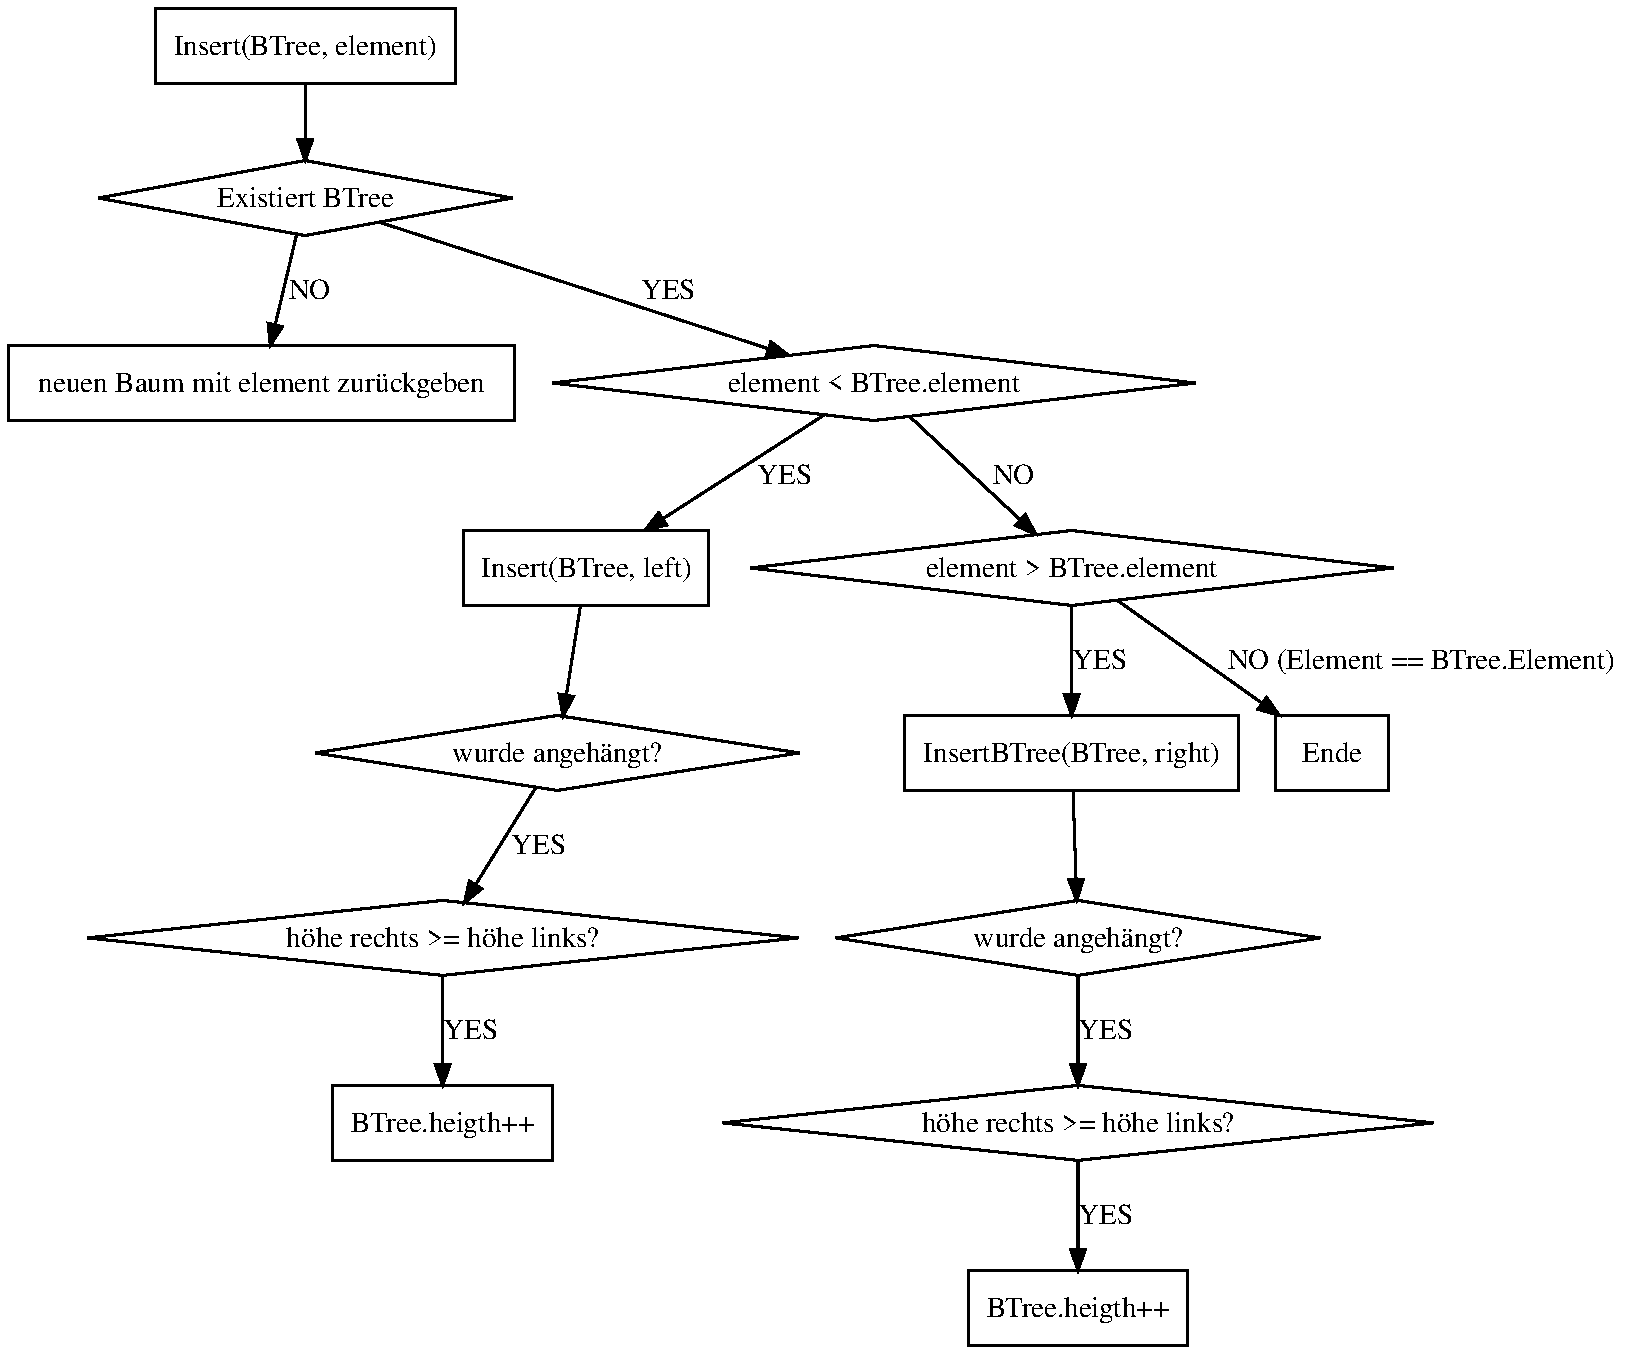
\includegraphics[width=1\columnwidth] {insert}
    \end{center}



    Fügt ein übergebenes Element einem übergebenem Baum hinzu. Zum Traversieren des Baumes wird bei jedem Schritt überprüft, ob das einzufügende Element kleiner oder größer dem derzeitigen Knoten-Element ist. Ist es kleiner geht man nach links, größer nach rechts. Die Höhe wird dynamisch angepasst. Ist ein leerer Platz gefunden, wird das Element dort eingefügt.

    \subsection{DeleteBT}

    \begin{center}
        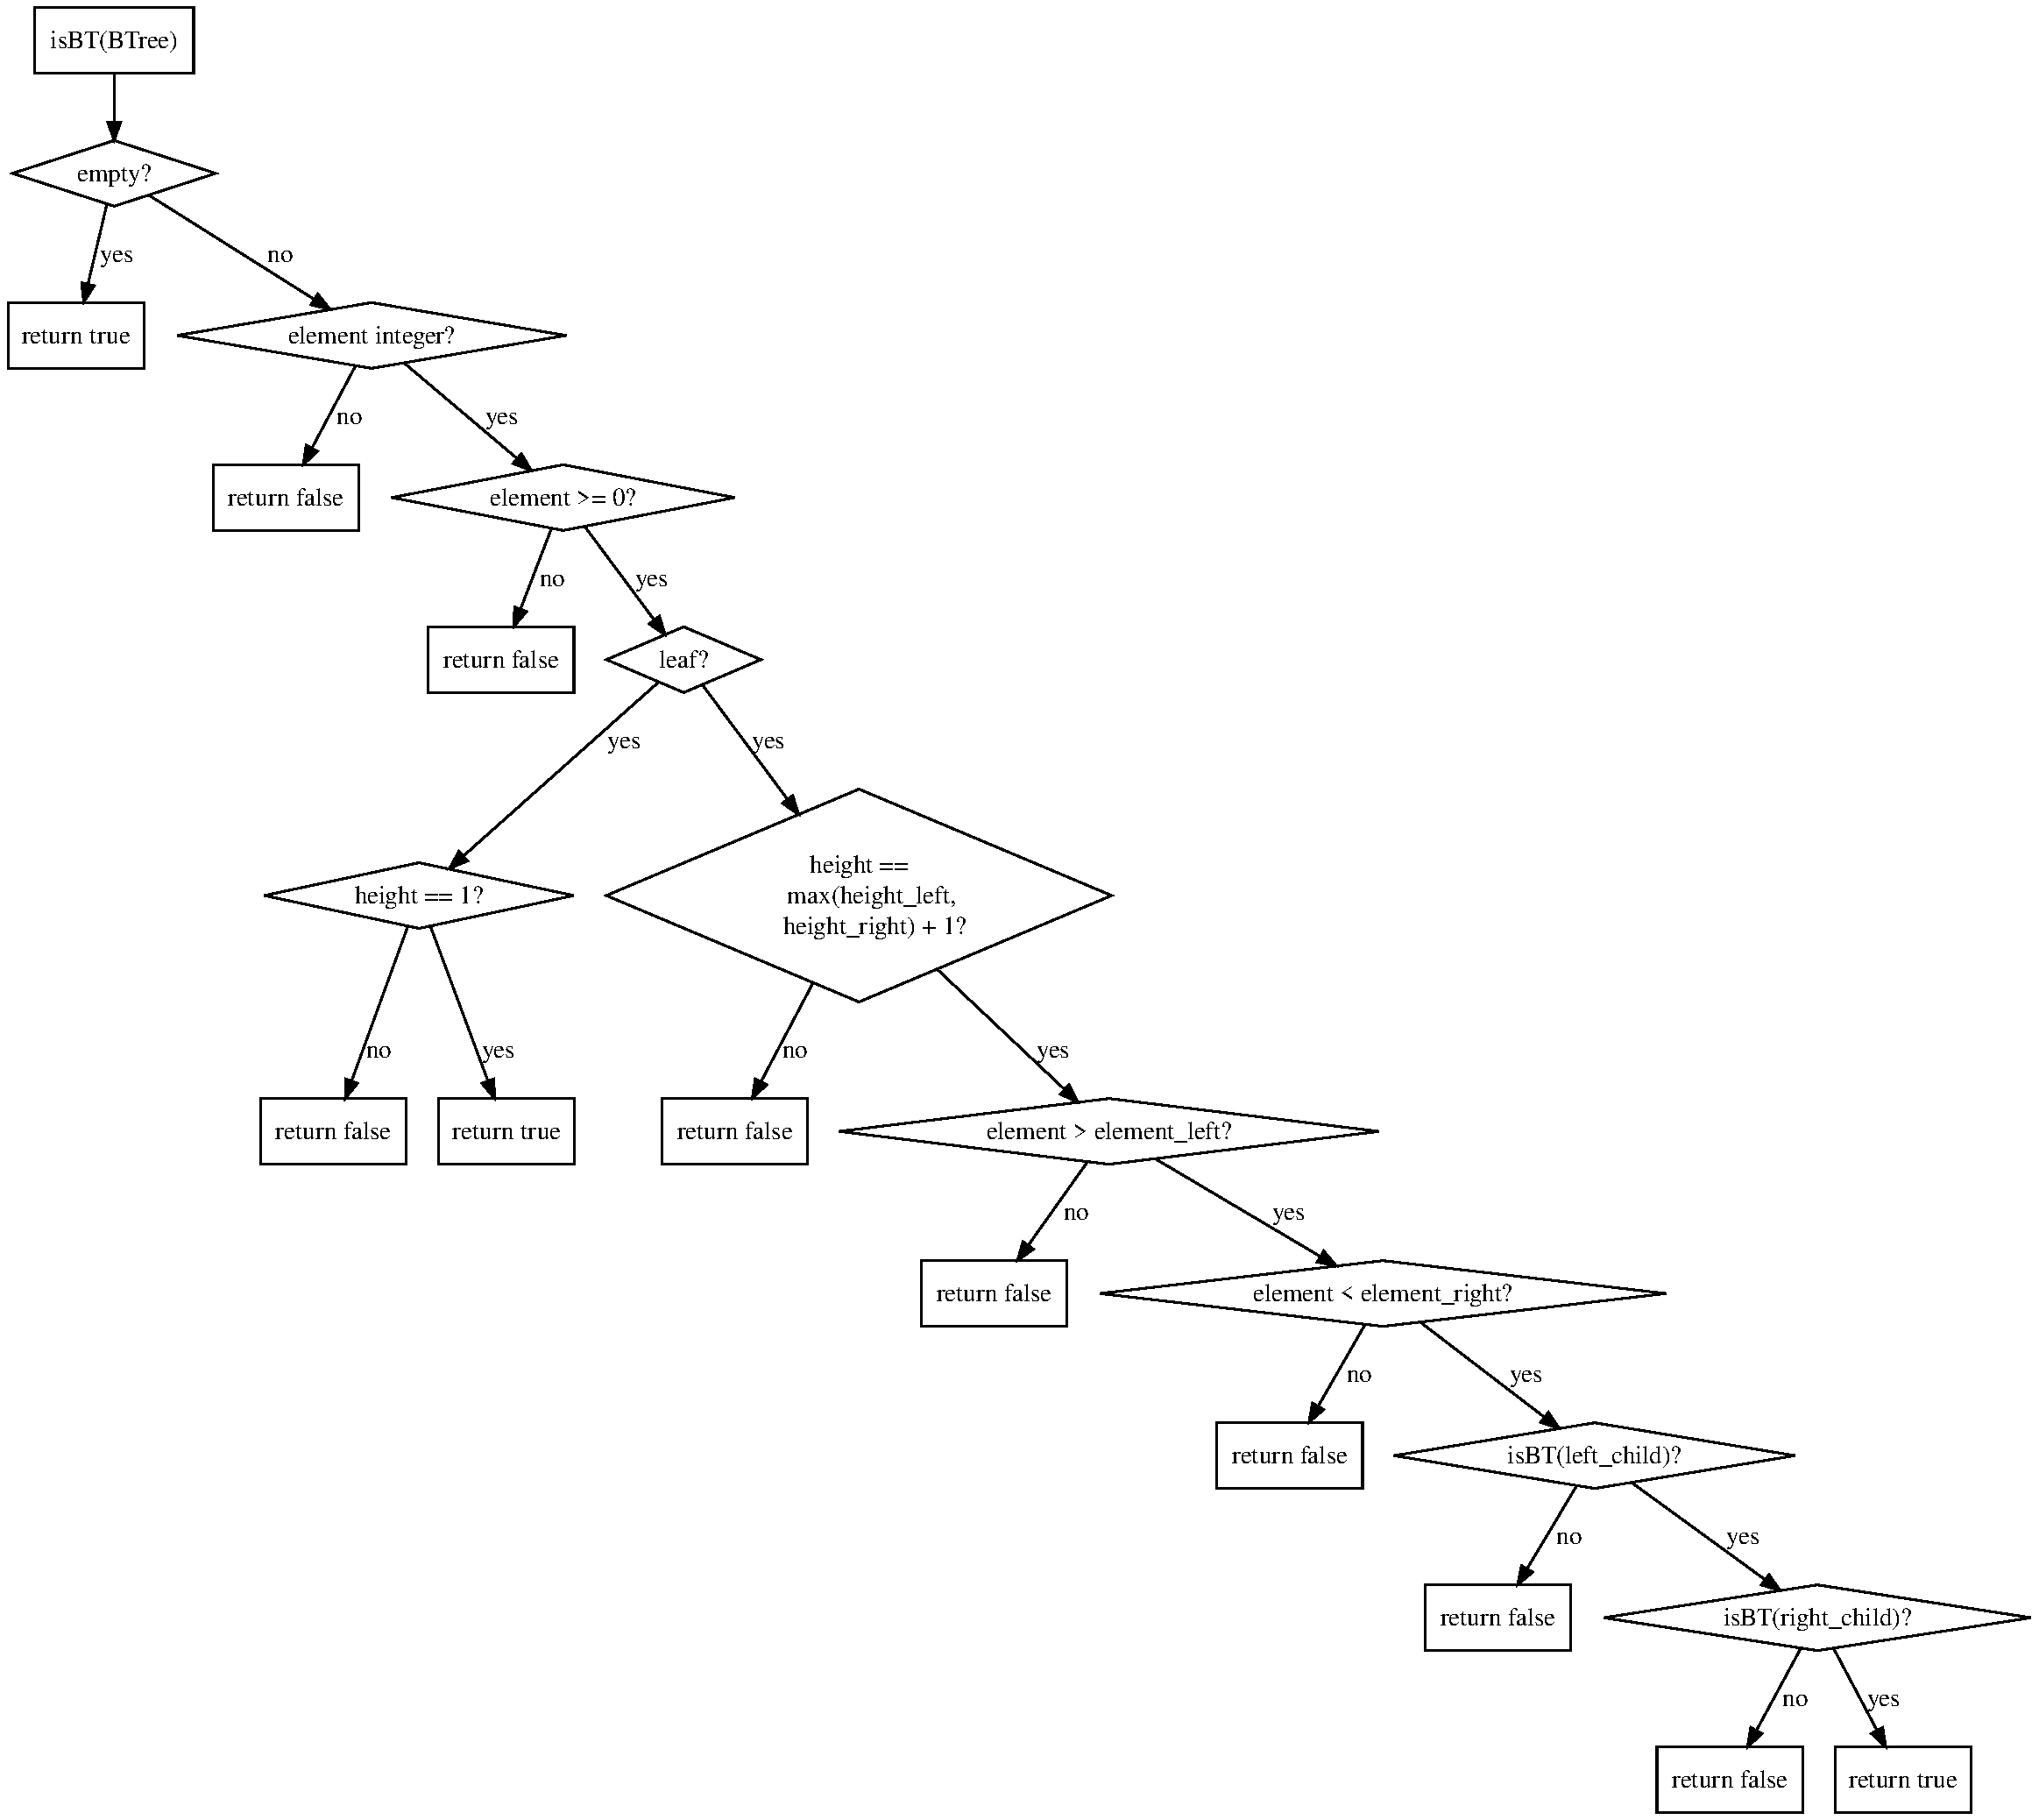
\includegraphics[width=0.8\columnwidth] {delete}
    \end{center}

    Löscht ein übergebenes Element aus einem übergebenem Baum. Traversierung des Baumes ist gleich wie in InsertBT. Ist das Ende des Baumes erreicht, ohne das Element gefunden zu haben, wird der Baum unverändert zurückgegeben. Wird das Element aufgefunden, kommt an seine Stelle das Element aus dem linken Teilbaum mit dem höchsten Wert. Die Höhe wird dynamisch angepasst.

    \subsection{Find}

    \begin{center}
        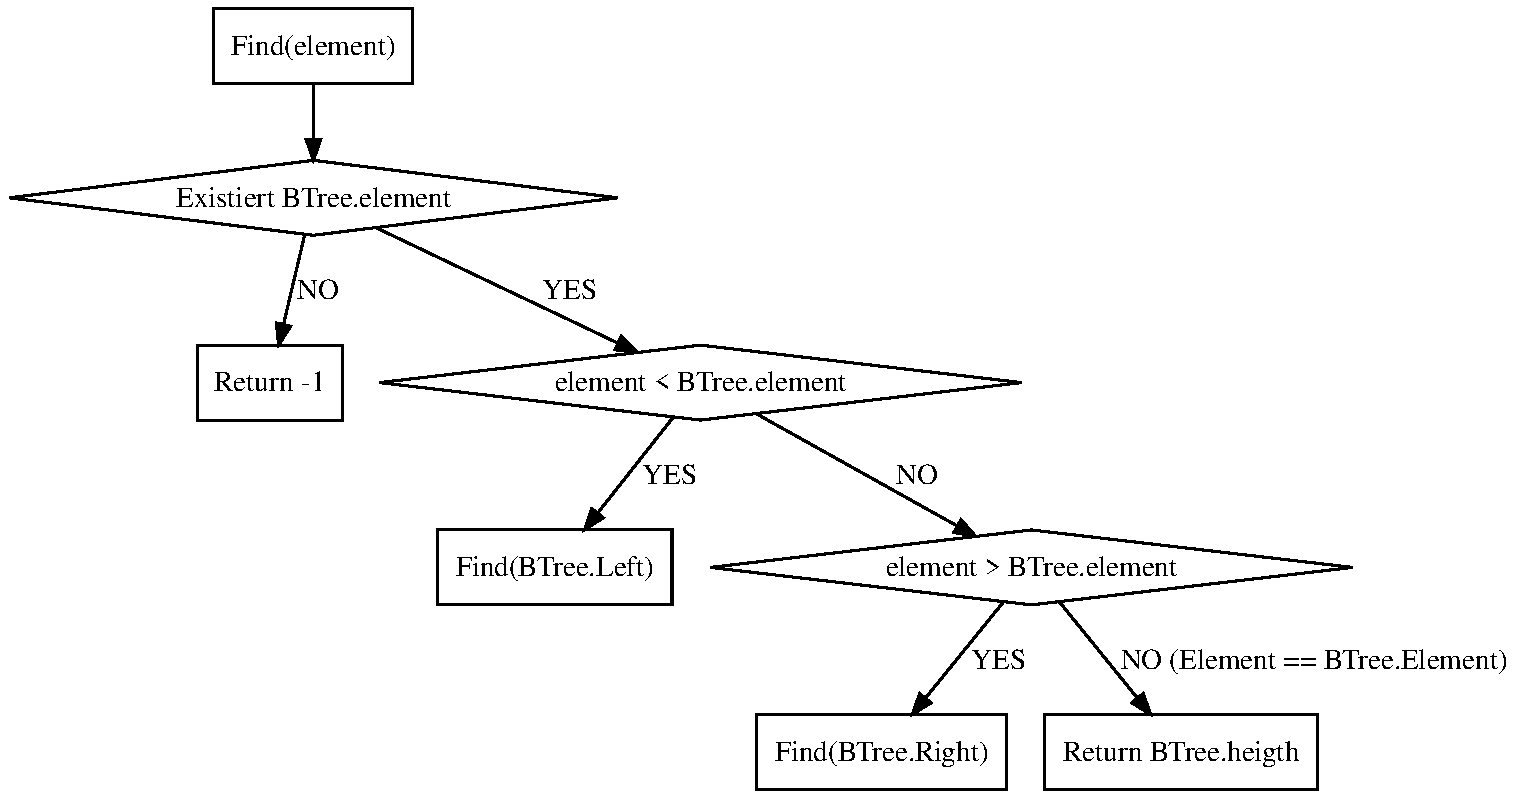
\includegraphics[width=1.1\columnwidth] {find.pdf}
    \end{center}

    Gibt die Höhe eines übergebenem Elements in einem übergebenem Baum aus. Traversieren des Baumes funktioniert hierbei gleich wie in InsertBT. Ist das Element gefunden, wird die Höhe des Knotens ausgegeben.

    \subsection{InOrderBT}

    \begin{center}
        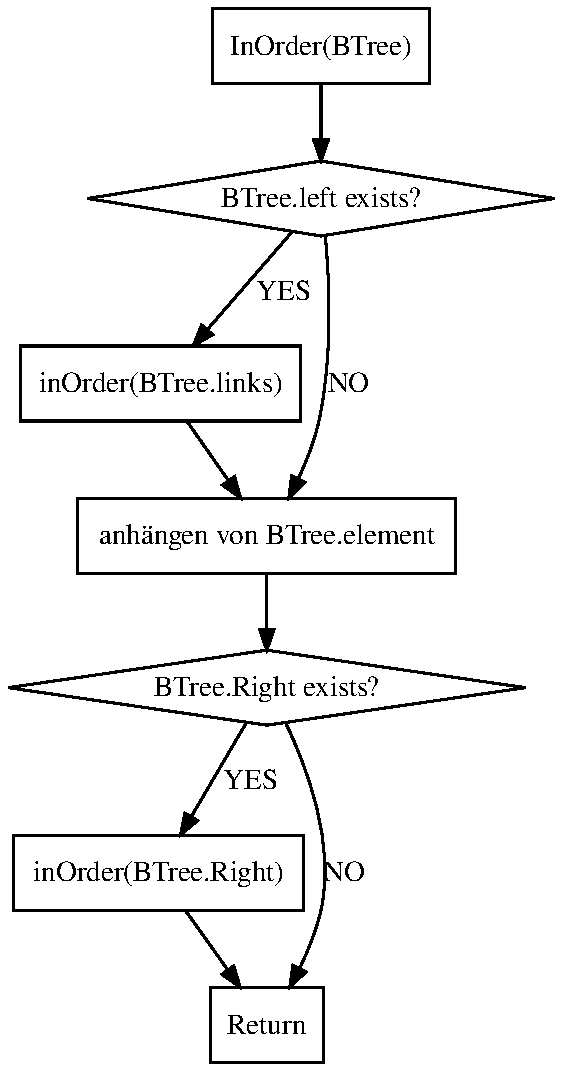
\includegraphics[width=0.4\columnwidth] {inorderhugo.pdf}
        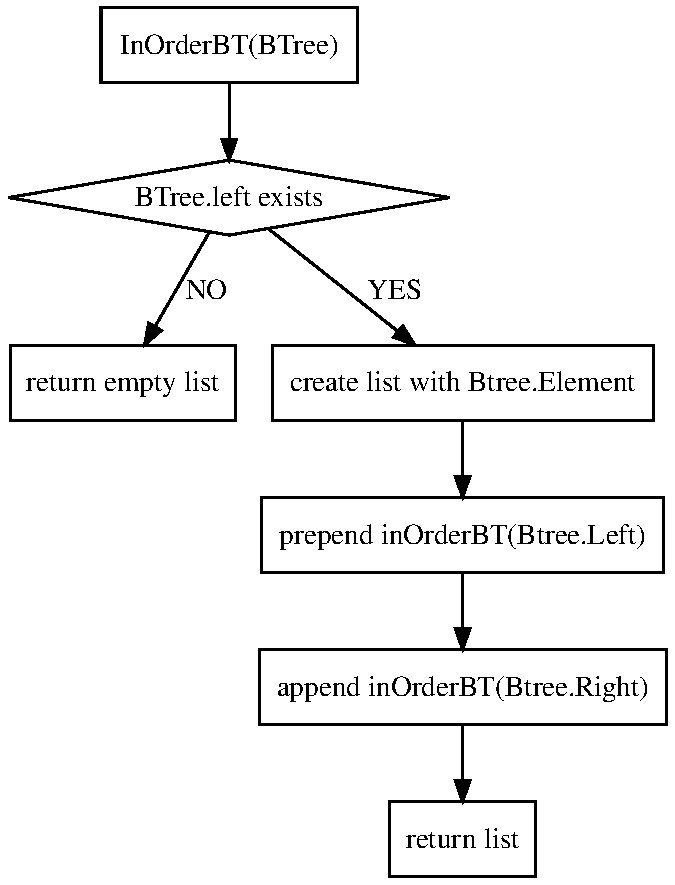
\includegraphics[width=0.5\columnwidth] {inorderjustin.pdf}
    \end{center}

    Gibt den Baum in Inorder in einer Liste aus. Es wird eine Liste mit dem Element des Knotens erstellt, wobei die Inorder des linken Kindes vorangestellt und die Inorder des rechten Kindes herangehängt wird. Ist das Ende des Baumes erreicht, wird eine leere Liste zurückgegeben. Hier haben wir zwei Optionen: Zum Einen kann bei jedem Funktionsdurchlauf der derzeitige Knoten selbst betrachtet werden (rechts). Zum anderen gibt es die Möglichkeit, bei der Überprüfung der Komponenten vorauszueilen und immer auf die Kinder des derzeitigen Knotens zu achten (links). Die Auswahl des Entwurfes ist implementationsabhängig.

\end{document}
